% --------------------------------------------------------------------------------------------------
\section{Discussion and concluding remarks}
Table \ref{table_discussion} presents the root-mean-square-error and computation time for each of 
the models presented in this report. Results show that adding Outer-Air-Temperature covariate does 
not improve significantly the fit to the model.

Model computed using XGBoost methodology as the minimum residual error and the faster computation 
time. The forecast using this model is attached in a separate file, as the prefered model.

\begin{table}[H]
\centering \begin{tabular}{c|cc}
                                    & RMSE & Computation time\\\hline\hline
SARIMA (without covariates)         &  8.60 &  56 min \\
SARIMA (with covariates)            &  8.31 &  1h16   \\
Neural Network (without covariates) & 14.93 &  1h10   \\
Neural Network (with covariates)    & 10.29 &  40 min \\
XGBoost (without covariates)        & 7.90  &  6 min
\end{tabular}
\caption{Root mean square error (RMSE) and computation time of modelling using different algorithms.}
\label{table_discussion}
\end{table}

\begin{figure}[!h]
\centering
 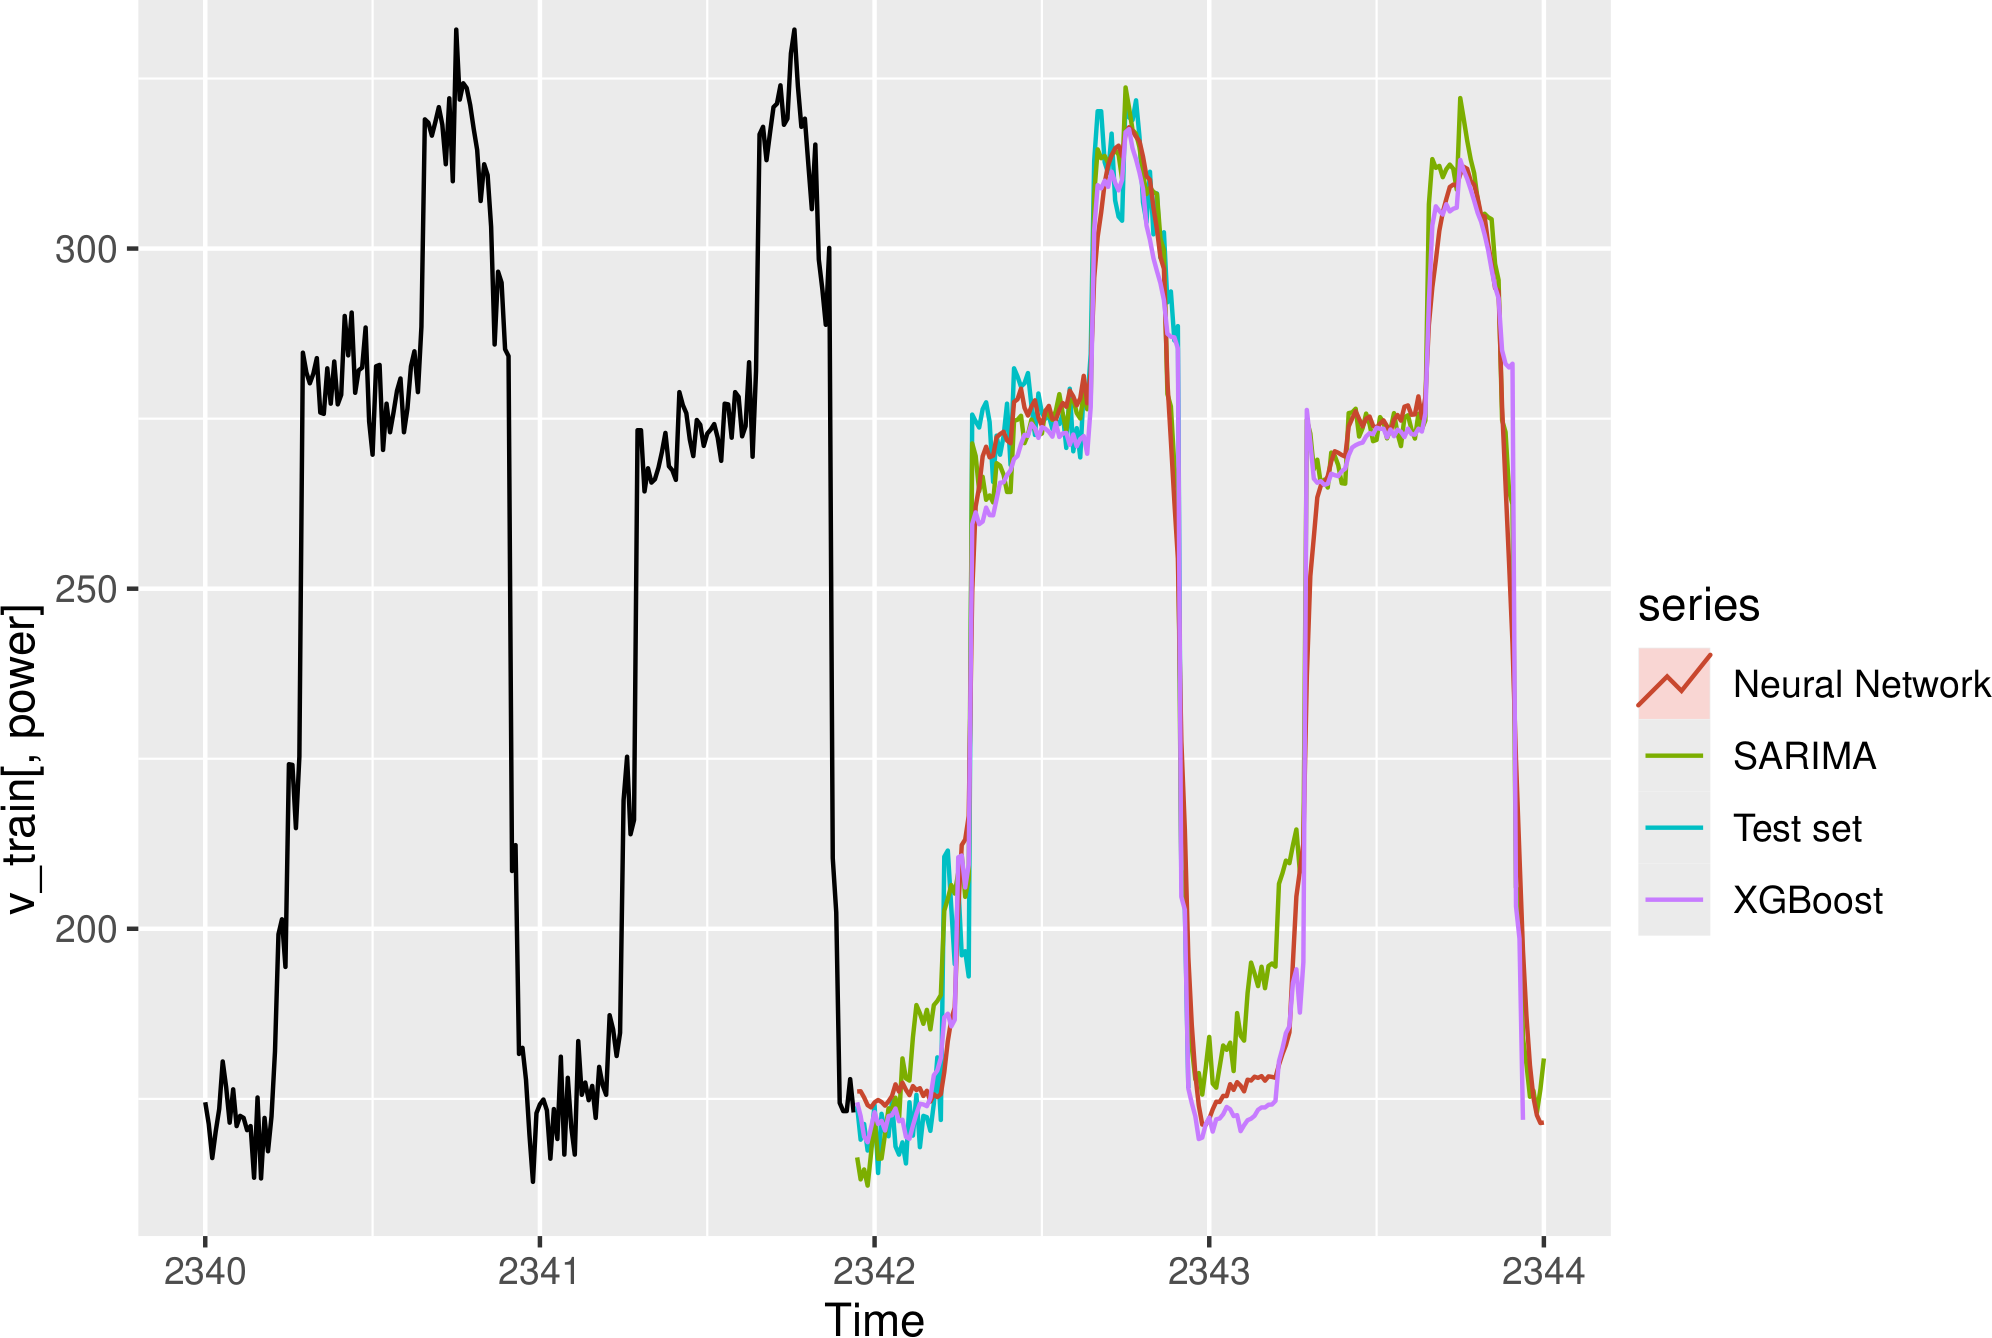
\includegraphics[scale=0.6]{figures/figure_discussion.png}
\caption{Modelling and forecast of electricity consumption using Outer-Air Temperature as a covariate.}
\label{figure_discussion}
\end{figure}

All R codes are available on Github (\url{https://github.com/JoanneAB/TimeSeriesForecasting}).

